% \documentclass[t, 10pt]{beamer}
\documentclass[t,handout, 10pt]{beamer}

\usepackage{graphicx}
\usepackage{epsfig}
\usepackage{psfrag}
\usepackage[english]{babel}
\usepackage{color}
%Mathematics packages
\usepackage{amsmath}
\usepackage{mathrsfs}
\usepackage{amsfonts}

\usepackage{enumerate}


\graphicspath{{./images/}} % Figures path - used in graphicx

\selectcolormodel{cmyk}

\mode<presentation>

%THEMES - Please refer to these chapters in the beamer documentation.
% Presentation themes : Chapter 15
% Color themes : Chapter 17
% Font themes : Chapter 18

\usetheme{Pittsburgh}
\usecolortheme{orchid}
\usefonttheme{default}

%---------------------------Title frame definition------------------------------------- 

\title{Policy-based Usage Management Overlay Networks}
\author [Greg, Chris]{Gregory Heileman and Christopher C. Lamb}
\institute[University of New Mexico]{
\inst {}Department of Electrical and Computer Engineering\\
University of New Mexico}
\date{}
\titlegraphic{
\begin{figure} 

\includegraphics[width = 7cm]{UNM}
\end{figure}}

% Delete this, if you do not want the table of contents to pop up at
% the beginning of each subsection:
%\AtBeginSubsection[]
%{
%  \begin{frame}<beamer>
%    \frametitle{Outline}
%     \tableofcontents[currentsection,currentsubsection]
%  \end{frame}
%}

\begin{document}

\begin{frame}
\titlepage
\end{frame}

% This command will make the logo appear on all frames excluding the title frame.
\logo {
\includegraphics[width = 2.5cm]{UNM}}

\begin{frame}
\frametitle{Introduction}
Today we will cover our work in usage management, new architectures we are developing to enable usage management, and how they apply to the cross domain information management problem.
\tableofcontents 
\end{frame}

\section{Usage Management}

\begin{frame}\frametitle{Usage Management}
\begin{itemize}
 \item \textbf{Usage management} refers to the ability to control how resources~(data and services) are used across and within computing domains.
 \pause
 \item Controlling how information is used becomes increasingly difficult as computing infrastructure becomes more distributed.  \pause However, the ability to share information between domains provides for powerful capabilities, as well as increased security risks.
 \pause
 \item Usage management incorporates aspects of access control and digital rights management (DRM):
 \pause
  \begin{itemize}
   \item Access control -- access rules are defined in terms of relationships between a set of resources and a set of users.
  \pause
  \item DRM -- access is implicit, the focus is on specifying and enforcing rules related to how the resource can be used.
  \end{itemize}
  \item We seek the development of open frameworks for usage management, based upon fundamental system design principles, that support interoperability within distributed computing environments. 
\end{itemize}
\end{frame}


\begin{frame}
\frametitle{Usage Management Meta-Model}
{\small
Fundamental design principle: \textbf{Policy and computing domain separation} --
 \centerline{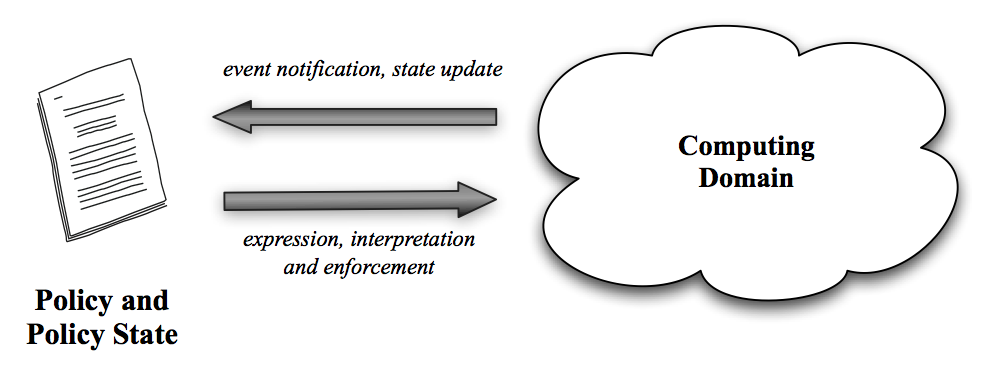
\includegraphics[width=3.5in]{meta-model.png}}
 \begin{itemize}
 \item A policy describes usage rules that govern how content may be used within computing domains.
 \pause
 \item The primary application of a policy is for reasoning whether or not a given action may be carried out within a given computing domain.
 \pause
 \item The current state of the policy (previous actions can affect this state), as well as the current conditions of the computing domain may be used in specifying usage rules.
 \end{itemize}}
\end{frame}

\begin{frame}\frametitle{Usage Management Meta-Model}
 \begin{itemize}
 \item Adherence to this design principle directly supports interoperability, and more specifically, the ability to operate across multiple computing domains.
 \pause
 \item Most of the ``policy" languages that have been proposed in the areas of access control and DRM can be mapped to this meta-model.
  \pause
 \item Based upon this meta-model we can identify the three major functionalities that a usage management framework must support: 
 \begin{enumerate}
  \item Policy Expression -- the usage rules.
  \item Policy Interpretation -- can an action be performed in a given domain?
  \item Policy Enforcement -- mechanisms for enforcing the allowed actions.
  \end{enumerate}
 \end{itemize}
\end{frame}

\begin{frame}\frametitle{A High-level UM Framework}
\begin{itemize}
\item We have created a usage management model based upon the meta-model that satisfies the previous separation principle through the interaction of two objects:
 \begin{itemize}
  \item[--] \textbf{Context Object} -- An instantiation of the ``context", i.e., the entities that exist within the computing domain, along with their relationships, and current state. 
  \pause
  \item[--] \textbf{License Object} -- Usage policies expressed in some program logic, along with the current policy state.
 \end{itemize}~\\
 \centerline{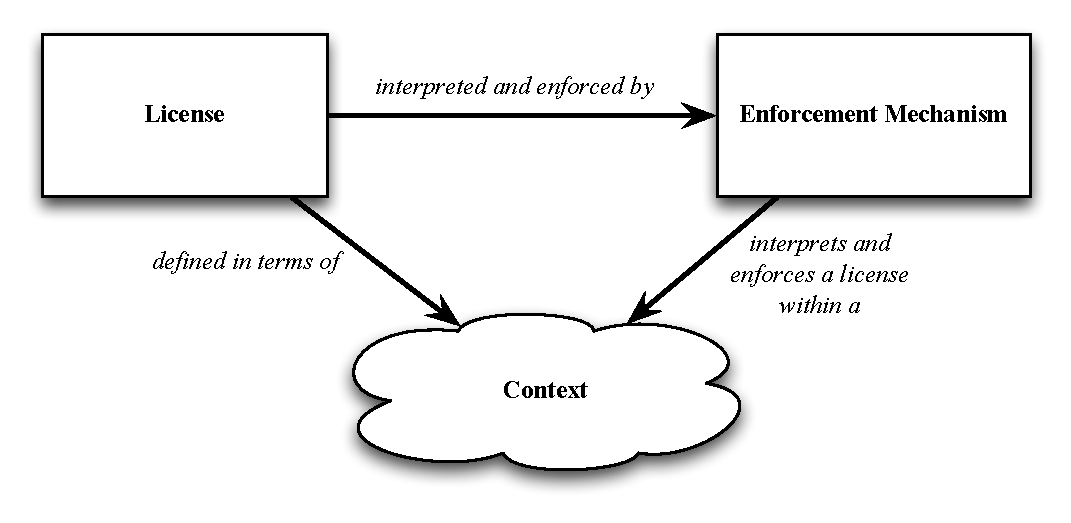
\includegraphics[width=3.5in]{model_overview.pdf}} 
 \end{itemize}
\end{frame}

\begin{frame}\frametitle{UM Framework -- Context Object}
  \centerline{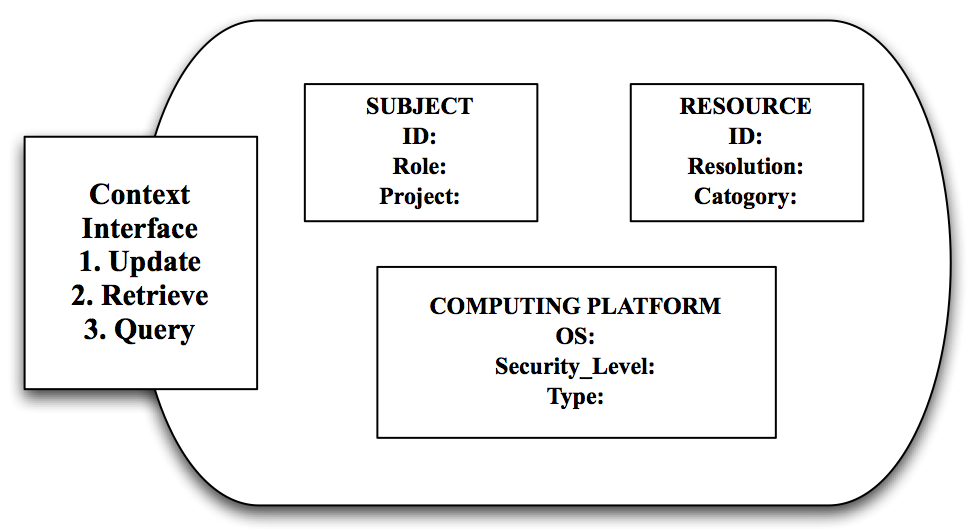
\includegraphics[width=2.5in]{context-obj.png}}
  \begin{itemize}
   \item Primary purpose: to capture the current conditions in the computation environment, and to provide them to the policy interpretation mechanism.
   \pause
   \item An update interface allows updating, retrieving and querying of the attribute values associated with the entities in the context.
   \pause
   \item A context object is updated by the system with appropriate values using the context interface.
  \end{itemize}
\end{frame}

\begin{frame}\frametitle{UM Framework -- Setup}
  \centerline{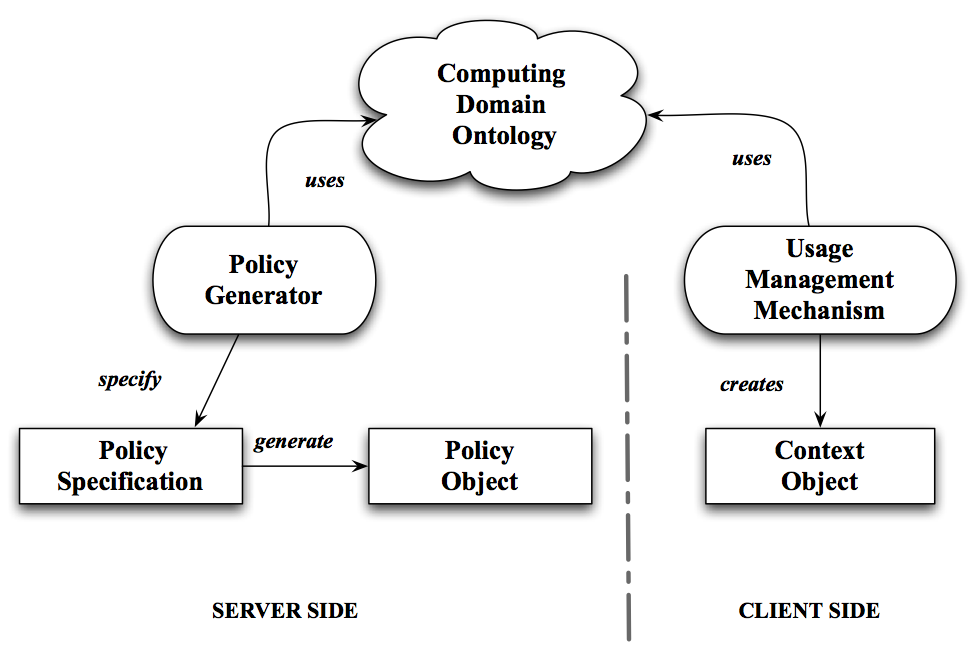
\includegraphics[width=3.5in]{UM-setup.png}}
    {\small Note: the policy interpretation and enforcement mechanisms have been rolled up into the usage management mechanism.}
\end{frame}  

  
\begin{frame}\frametitle{UM Framework -- Operation}
  \centerline{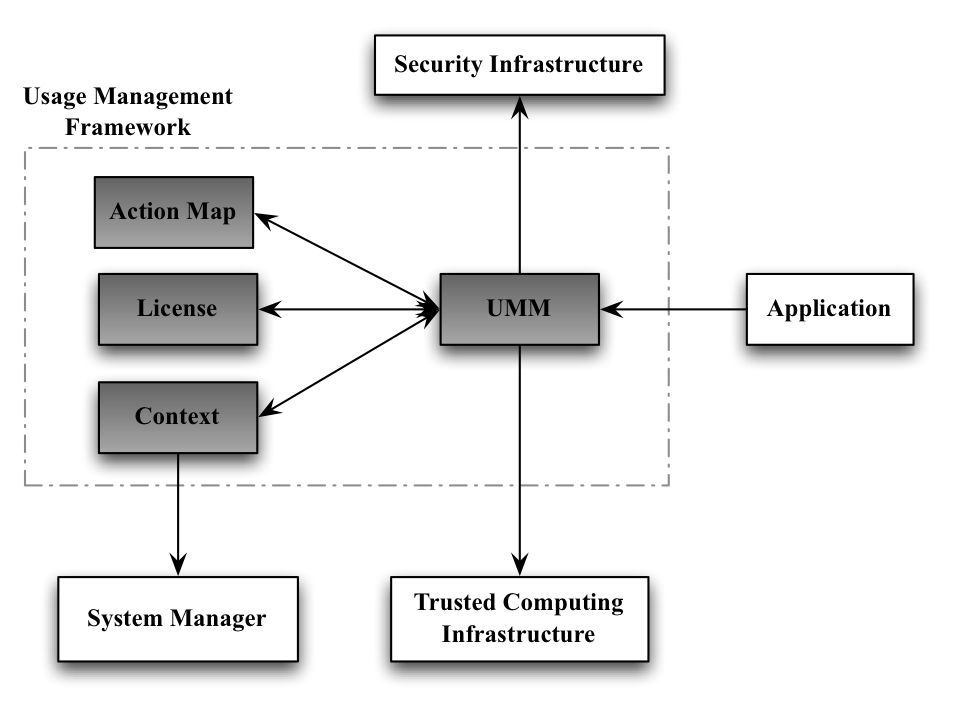
\includegraphics[width=3.75in]{UM-operation.png}}
\end{frame}  

\begin{frame}\frametitle{UM Framework -- Operational Semantics}
\vspace*{-0.1in}
  \centerline{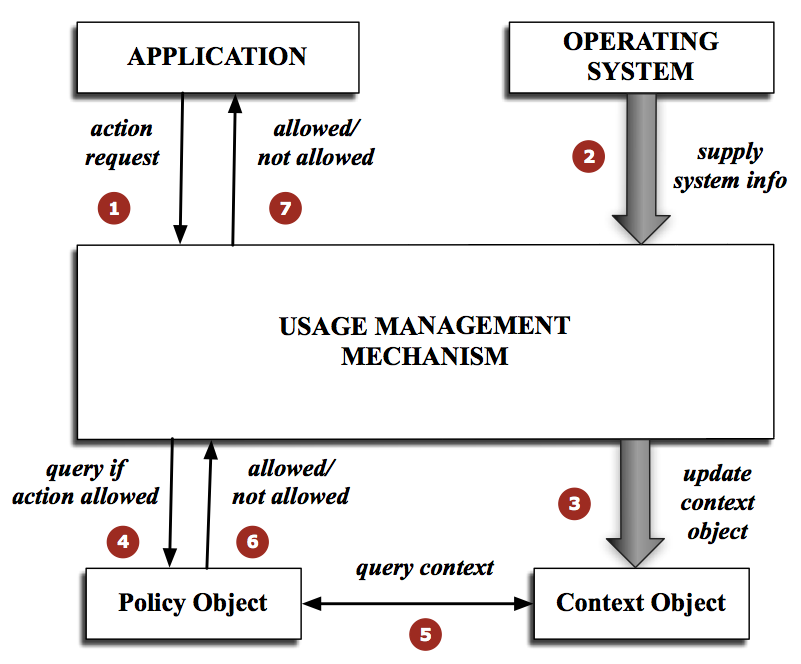
\includegraphics[width=3.25in]{UM-working.png}}
  {\small Note:  the operational semantics of the framework are independent of syntax and semantics of any particular type of policy languages or logics.}
\end{frame}  
  
\begin{frame}\frametitle{UM Framework -- Cross-domain}
~\\  \centerline{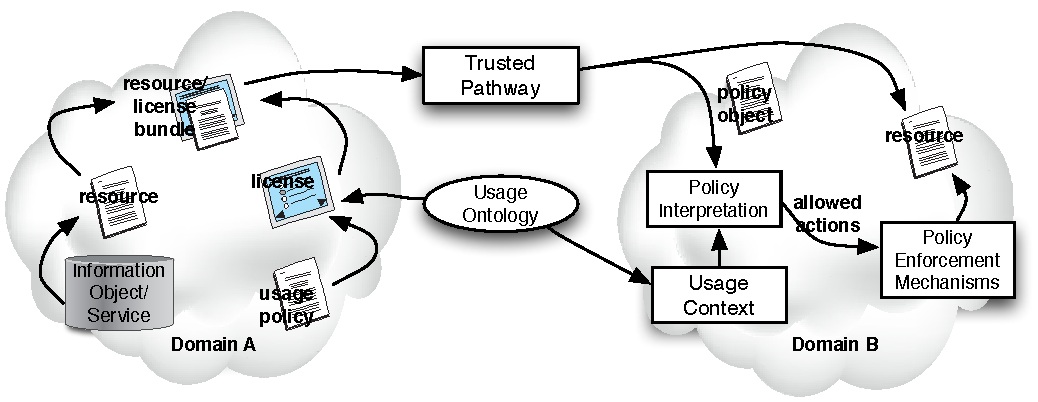
\includegraphics[width=4.25in]{UM-highlevel.pdf}}~\\
  {\small Note: this is one possible high-level architectural realization of the UM model that is meant to depict the pieces necessary in each domain, along with their dependencies. These are NOT data flows.}
\end{frame}  

\section{Scenarios}

\begin{frame}
\frametitle{Applicable Scenarios}
In order to demonstrate the flexibility of our approach, we will work through a series of possible scenarios with regard to sensitive information dissemination and use.
\newline
\pause
\begin{itemize}
\item \textbf{Go back to class!}
\pause
\item \textbf{Changes roll downhill}
\pause
\item \textbf{Operational Chaos}
\end{itemize}
\end{frame}

\begin{frame}
\frametitle{Scenario 1: Go Back to Class!}
Imagine a new cabinet secretary is appointed.  Shortly thereafter, the new secretary  unclassifies swathes of information - documents, presentations, data sets, you name it.  Well, no secretary is forever, so eventually that secretary moves on and a new one comes in.  That new secretary is appalled at the open flow of information in his agency and immediately clamps down, reclassifying oceans of documents.
\newline
\newline
Results of this change include:
\newline
\pause
\begin{itemize}
\item \textbf{Lost Time} --- Agency personnel and contractors spend significant portions of their lives remarking documents...
\pause
\item \textbf{Inaccuracy} --- ...and despite their best efforts, humanity rears it's ugly head in the form of reams of mismarked information that takes years to sort out.
\end{itemize}
\end{frame}

\begin{frame}
\frametitle{Scenario 1: Core Problem}
So why did so many people need to sacrifice so much time to reclassify previously released information?
\newline
\pause
\begin{center}
\textbf{Hierarchical Mismatch.}
\end{center}
\pause
Here, we have one one side a clear organizational hierarchy, spanning from the secretaries down to those who actually needed to clean up the messes those hypothetical secretaries made.  On the other, we have a mass of essentially undifferentiated documents with embedded security metadata.
\end{frame}

\begin{frame}
\frametitle{Scenario 1: Policy/Content Separation}
One way to address this problem is by separating the \textbf{content} we're protecting from the \textbf{policies} describing how that content can be used.
\pause
\newline
\newline
This gives us \textbf{indirection} between policy and content, allowing us to be more flexible with how policies are managed.
\pause
\newline
\newline
We could organize policies in a clear hierarchy, where content classifications can be defined one once, in policies within that hierarchy, rather than innumerable times within classified documents.
\end{frame}

\begin{frame}
\frametitle{Hierarchical Policy Solution}

\begin{columns}[T]
\begin{column}{5cm}
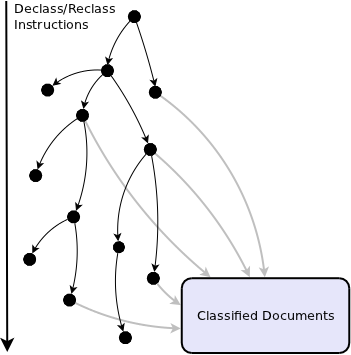
\includegraphics[width=4cm]{hierarchy-1}
\newline
\newline
Classification Propogation without Policies:
\newline
\begin{itemize}
\item \textbf{Everyone involved}
\item \textbf{Lost time}
\item \textbf{Wasted Funds}
\end{itemize}
\end{column}
\begin{column}{5cm}
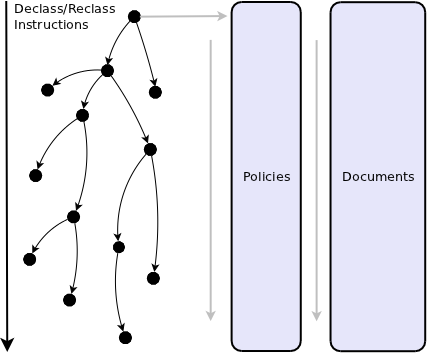
\includegraphics[width=5cm]{hierarchy-2}
\newline
\newline
Policy-based management:
\newline
\begin{itemize}
\item \textbf{Less change required}
\item \textbf{Policy hierarchy does the work}
\end{itemize}
\end{column}
\end{columns}

\end{frame}

\begin{frame}
\frametitle{Scenario 2: Changes Roll Downhill}
Scenario 1 shows the use of top-down control of a given group of policies.  If top-down is effective, can we have similar advantages from a bottom-up use of a policy hierarchy?
\pause
\newline
\newline
\textbf{Yes, we can.}
\pause
\newline
\newline
Imagine a case where an organization:
\begin{itemize}
\item \textbf{... is working with an untrusted partner} --- Say, for example, some coalition partner that is not entirely trusted with all the intelligence a given organization may have about a situation.
\item \textbf{...must limit information access} --- Not only by content, but perhaps by other factors like time.
\item \textbf{...must be able to retract access} --- Access to information needs to be retracted after a given time window.
\end{itemize}
\end{frame}

\begin{frame}
\frametitle{Scenario 2: Core Problem}
The problem here is somewhat different from that presented in the first Scenario.
\newline
\newline
\pause
Here we have:
\begin{itemize}
\item \textbf{Unequal information sharing} ---  Partners do not have the same access as organizational members.
\item \textbf{Decisions made on the basis of content and context} --- Decisions are made based on dynamic conditions, including the current reputation of the partner and the type of information accessed.
\item \textbf{Decisions made close to the sharing scenario} --- These decisions need to be made frequently by those most familiar with immediate use of the information and the context of use.
\end{itemize}
\end{frame}

\begin{frame}
\frametitle{Scenario 2: Bottom-up Locality}
\textbf{This gives us a certain degree of \textit{bottom up locality}.}
\newline
\newline
\pause
In this case, we have:
\pause
\begin{itemize}
\item \textbf{Decisions made close to operational environment} --- Access decisions must be made frequently with knowledge of local context.
\pause
\item \textbf{Locality of leadership vital} --- Frequency of decisions and dynamic nature of context preclude decision-from-a-distance.
\end{itemize}
\end{frame}

\begin{frame}
\frametitle{Scenario 2: Hierarchical Mirroring}
\begin{columns}[T]
\begin{column}{5cm}
Separation of \textbf{policy} from \textbf{content} at this level allows local decisions.
\newline
\newline
Decisions can be made at multiple levels based on local contexts, propagating to vital parties quickly.
\end{column}
\begin{column}{5cm}
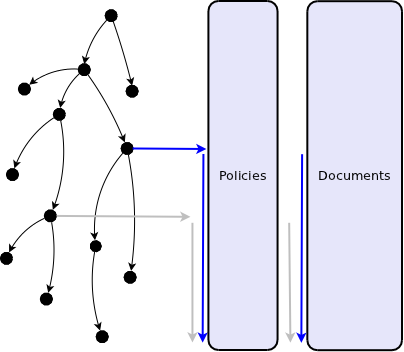
\includegraphics[width=5cm]{hierarchy-3}
\end{column}
\end{columns}
\end{frame}

%\begin{frame}
%\frametitle{Test}
%
%\begin{columns}[t] 
%\begin{column}{5cm}
%Two\\lines.
%\end{column}
%\begin{column}{5cm}
%One line (but aligned).
%\end{column}
%\end{columns}
%
%\end{frame}

\begin{frame}
\frametitle{Scenario 3: Operational Chaos}
Under common conditions, technology and communications equipment is not very effective.  These kinds of situations occur regularly under the stress of catastrophic conditions, for example.
\newline
\newline
\pause
These conditions generally share certain characteristics:
\begin{itemize}
\item \textbf{Dynamic operations} --- The communication and computer operational networks have very dynamic topologies where groups are unexpectedly isolated and then reconnected.
\pause
\item \textbf{System breakdown} --- Systems tend to breakdown unexpectedly and catastrophically.
\pause
\item \textbf{Centralized systems unavailable} --- As a result of communication breakdowns, centralized systems become unavailable or unreliable.
\end{itemize}
\end{frame}

\begin{frame}
\frametitle{Scenario 3: Core Problem}
As communications becomes less reliable, information becomes more valuable and highly demanded.
\newline
\pause
\begin{itemize}
\item \textbf{Need information in high stress environments} --- Information demand increases under stress as those involved demand more situational awareness.
\pause
\item \textbf{Communication capabilities highly variable} --- Communications capabilities decrease as systems are destroyed or otherwise go offline leading to unreliable infrastructure.
\pause
\item \textbf{Must operate under attack} --- Even though the conditions are hostile, systems \textbf{must} provide some level of service and degrade gradually if at all in extreme environments.
\end{itemize}
\end{frame}

\begin{frame}
\frametitle{Scenario 3: Information Management Cells}
Under these conditions, end-to-end principles in system design can provide the appropriate scalability and reliability to support continued operations under stress.  
\begin{center}
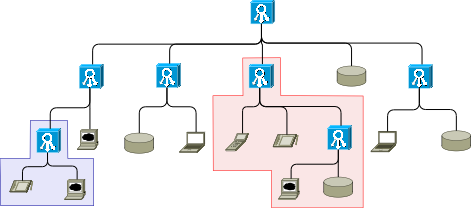
\includegraphics[width=7cm]{info-cells}
\end{center}
End-to-end design provides:
\begin{itemize}
\item \textbf{Stalability, Reliability, Perfomance} --- Complex nodes, simple core
\item \textbf{Exploits Locality} --- Centralized queries offline, local still available
\end{itemize}
\end{frame}

\section{Analysis}

\begin{frame}
\frametitle{Underlying Characteristics}
What are the underlying principles that enable this flexibility?
\pause
\begin{itemize}
\item \textbf{Separation of Concerns} --- Specifically, we separate \textbf{policy} from \textbf{content}.
\pause
\item \textbf{End-to-End principle application} --- As we move away from centralized cross-domain guards we push functionality closer and closer to content.  We also begin to create distinct usage management cells, enabling \textit{collaboration over centralization}.
\pause
\item \textbf{Dynamic Context} --- Context change radically in the context of artifact use.  Environmental conditions that forbid access to information content can change gradually or quickly, leading to conditions under which that content must be widely accessed.
\pause
\end{itemize}
\end{frame}

\begin{frame}
\frametitle{Separation of Concerns}
How does separation of concerns help us?
\newline
\newline
\pause
Why does it help in other domains? Say Javascript/CSS/HTML?
\begin{itemize}
\item \textbf{Rates of change} --- Some things change at different rates.  In web development, content (HTML) may stay the same, but the presentation (CSS) of the content will change.  Likewise, the presentation may be static, but the behavior (Javascript)  may need to evolve.
\item \textbf{Roles} --- Different roles may be suitable for different types of work.  Here, content may be edited near constantly, while the presentation of that content may be static.
\end{itemize}
\pause
In usage management scenarios, we have similar issues.
\end{frame}

\begin{frame}
\frametitle{End-to-End Principles}
How do end-to-end principles help us?
\newline
\newline
\pause
End-to-End principles were originally outlined to help design forerunner networks to what we now know as the internet.
\newline
\newline
\pause
Essentially, they encourage simplicity in the core switching fabric of a network with application complexity pushed out to nodes in a network graph.
\newline
\newline
\pause
Although recent approaches have abandoned these ideas, they have done so at the price of loss of scalability, reliability, and performance.
\end{frame}

\begin{frame}
\frametitle{Dynamic Context}
How does recognition of dynamic contexts help us?
\newline
\newline
\pause
We know that environments and situations change, and change rapidly.  Not recognizing this leads to brittle systems that are prohibitively expensive to maintain, if they work at all.
\newline
\newline
\pause
With dynamic context support we can:
\begin{itemize}
\item \textbf{Retract access based on conditions} --- Simply recognizing a larger context enables the system to automatically restrict access to sensitive material based on changing conditions.
\pause
\item\textbf{Map \textit{activities} to \textit{actions}} --- Reading a document may in fact not be a single activity, but rather a sequence of actions (lookup, retrieve, save, open, display) that are managed separately in certain situations.
\end{itemize}
\end{frame}

\section{Prototype Results}

\begin{frame}\frametitle{Prototype Demonstration}
\vspace*{-0.1in}
  \centerline{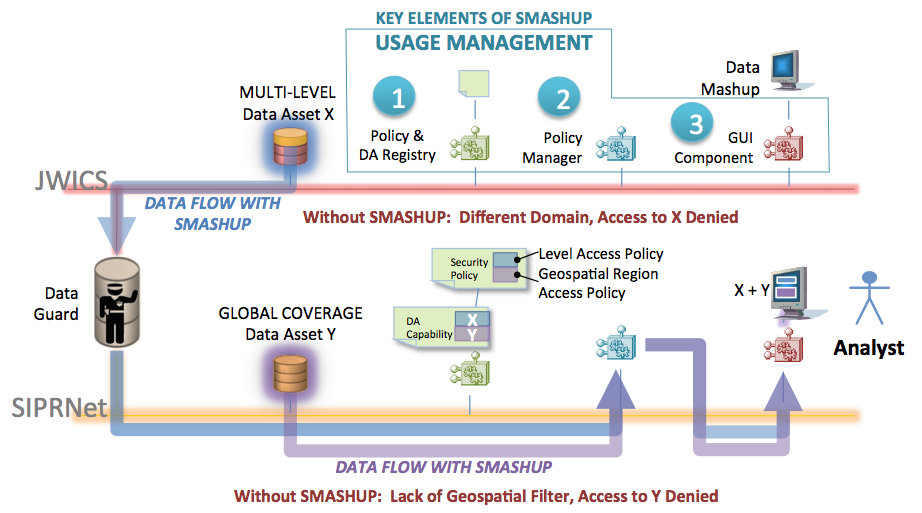
\includegraphics[width=4.35in]{demo.png}}
  {\small Note:  the guard functionality in this demonstration was not a separate module, and was provided as part of usage management framework.}
\end{frame} 

\begin{frame}\frametitle{Prototype Demonstration -- Capabilities}
{\small
The Phase I prototype demo was used to exhibit the following capabilities:
\begin{itemize}
\item Licenses that contained policies expressing both access and usage control rules were constructed to enable persistent information security over data elements.
\pause
\item The concept of a license being interpreted in real-time according to the current
context was exhibited.
\pause
\item The capability of real-time aggregation of licenses, and reasoning over the resulting
combined policies was demonstrated. This included situations were polices precluded certain data elements from being mixed together, and the reasoning about this occurred in real-time, as the mashup was being constructed.
\pause
\item Information sources belonging to different realistic DoD security domains, and the sharing of objects between them, were simulated (there was no communication through any type of trusted pathway though), taking into account the roles of the personnel involved, the devices they were using, etc.
\end{itemize}}
\end{frame}

\begin{frame}\frametitle{Prototype Demonstration -- Limitations}
{\small
The Phase I prototype demo was limited in the following ways:
\begin{itemize}
\item The demo did not provide a formal ontology for the domain. Rather this was ``hard- coded" into the demo.
\pause
\item User authentication was simulated.
\pause
\item Although access to data sources was dynamically computed according to policy, the
data sources themselves were static. I.e., map data was not generated by a database query, but rather was stored as fixed images. 
\pause
\item It did not provide a mechanism for generating licenses using an underlying ontology; XML licenses were constructed ``by hand."
\pause
\item The logic associated with reasoning over license aggregation was very simplistic, essentially a logical ANDing over the license terms.
\pause
\item The semantics of the licenses were also rudimentary, e.g., only permissions were considered, not obligations, usage history, etc.
\end{itemize}}
\end{frame}

\begin{frame}\frametitle{Prototype Demonstration -- Limitations}
{\small
\begin{itemize}
\item Reasoning over the interoperability of licenses between different domains was not considered. With a formal notion of interoperability, one context (domain) can query another, in order to determine if the other domain is able to interpret a particular policy.
\pause
\item The demo did not exhibit the capabilities of dynamic interpretation, where one activity specified in a license could lead to different actions depending upon the environment in which it is being interpreted.
\pause
\item The security of the system was not rigorously evaluated against any type of threat model. If we can formally capture a threat model, then we can better understand how usage management plays in the architecture. (AFRL help would be appreciated here.)
\pause
\item The trusted pathway was not a stand-alone entity. We implicitly supplied one through our usage management mechanism, thereby providing a distributed cross-domain sharing solution.
\pause
\item Query capabilities over usage scenarios (i.e., what led to a particular rule in a combined license) were not provided.
\end{itemize}}
\end{frame}


\section{Conclusions}

\begin{frame}
\frametitle{Conclusions and Future Work}
We have developed initial systems embodying these concepts.
\newline
\newline
\pause
Currently, additional distributed systems are in development that will apply these ideas to XML and HTML/RDFa content using HTTP-centric protocols.
\newline
\newline
\pause
Additional future areas of study include migration of these ideas into the core of cloud systems (e.g. Eucalyptus), application to addtional domains (e.g. medicine)
\end{frame}

\end{document}

